

\chapter{FIR}

\section{Window Method}

\subsection{Low Pass Design}

In this example, we design a low pass FIR filter using 2 windows: rectangular and Hamming.\\

The rectangular provides the best transition bandwidth, but has unacceptable ripples in the pass band and the stop band, so we use Hamming window to adjust these unacceptable ripples in the expense of a wider transition bandwidth.\\

The design specifications are:

\begin{itemize}
    \item Order: 24
    
    \item Normalized cuttoff frequency: 0.5
\end{itemize}

\newpage
Results are in \autoref{fig:FIR_Sim:FIR_lowpass_rect_Hamm_window}.

\begin{figure}[ht]
\centering
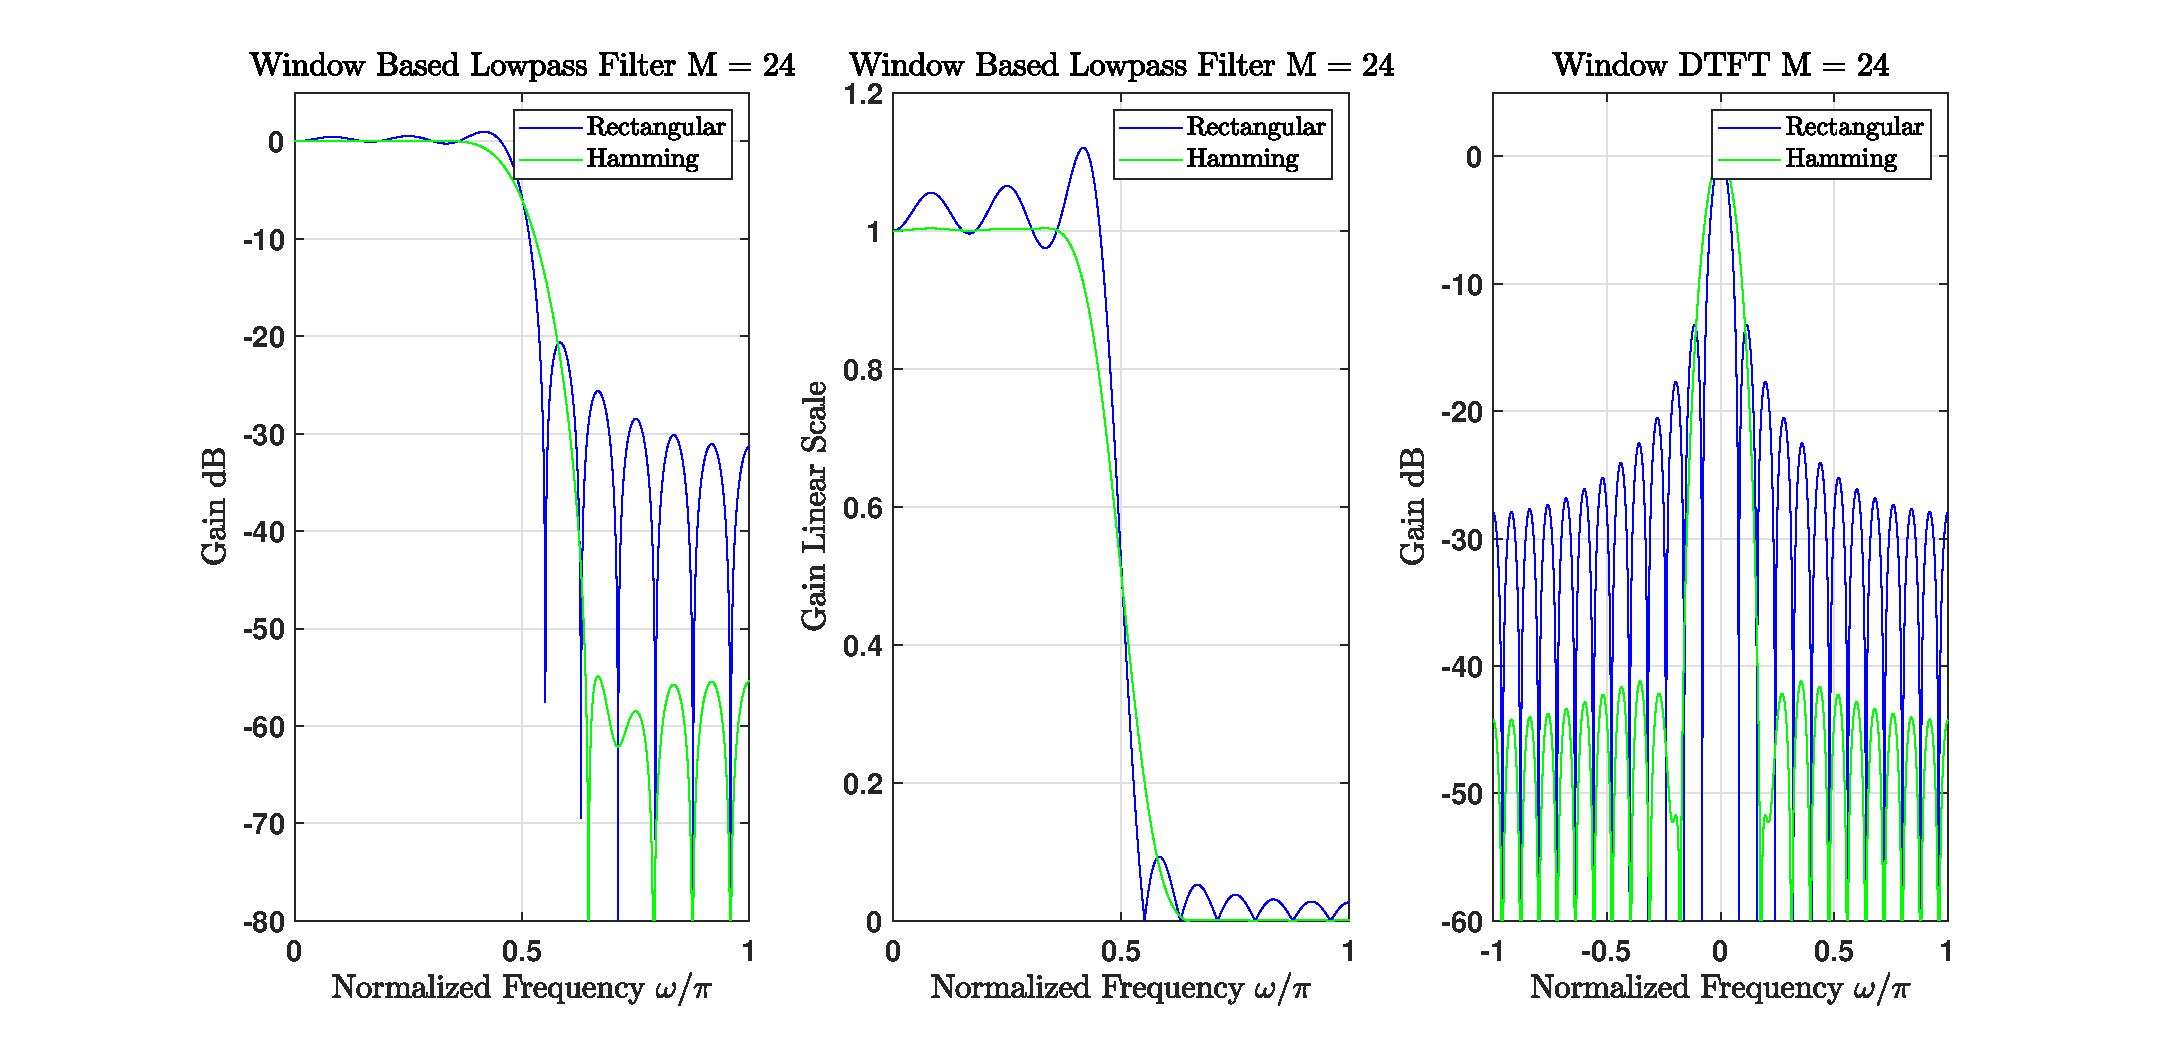
\includegraphics[scale = 0.5]{Figures/FIR_Sim/lowpass_window_method.eps}
\caption{FIR Low pass example using Rectangular and Hamming window}
\label{fig:FIR_Sim:FIR_lowpass_rect_Hamm_window}
\end{figure}

\begin{itemize}
    \item For Hamming window:
    
        \begin{itemize}
            \item Main lobe width is $\displaystyle\frac{8 \pi}{M}$ where $M$ is the filter order in this case
            
            \item Peak side lobe is -41 dB
        \end{itemize}
    
    
\end{itemize}

\subsection{Bandpass Design}

Now we will do a banpass design using the following specs shown in \autoref{fig:FIR_Sim:bandpass_example_given}

\begin{figure}[ht]
\centering
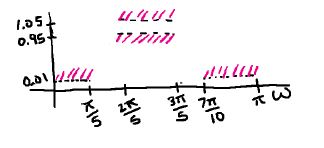
\includegraphics[scale = 0.7]{Figures/FIR_Sim/bandpass_example_given}
\caption{Bandpass Design Example}
\label{fig:FIR_Sim:bandpass_example_given}
\end{figure}

\begin{itemize}
    \item In the $\mathrm{1}^\mathrm{st}$ stop band, the transition bandwidth is $\displaystyle\frac{2 \pi}{5} \, - \, \displaystyle\frac{\pi}{5} \, = \, \displaystyle\frac{ \pi}{5}$
    
    \item In the $\mathrm{2}^\mathrm{nd}$ stop band, the transition bandwidth is $\displaystyle\frac{7 \pi}{10} \, - \, \displaystyle\frac{3\pi}{5} \, = \, \displaystyle\frac{ \pi}{10}$
    
    
    \item So as a result and specification we choose the smaller transition bandwidth that is $\displaystyle\frac{ \pi}{10}$
    
    \item As a deviation error, we have  $0.01 < 0.05$, so we take 0.01 as the error to be computed in the stopband and the bandpass
    
    
\end{itemize}

The window to be chosen for the specification is the Kaiser window, which depends upon 2 parameters:

\begin{enumerate}
    \item $\beta$ which controls the window shape: if $\beta \, = \, 0 \rightarrow$ rectangular window, and if $\beta$ increase then the mainlobe width increase and the sidelobe height decrease
    
    \item $M$ for the transition bandwidth
    
\end{enumerate}

\newpage
Results are shown in \autoref{fig:FIR_Sim:bandpass_Kaiser_results} and \autoref{fig:FIR_Sim:bandpass_example_error_plot}.

\begin{figure}[ht]
\centering
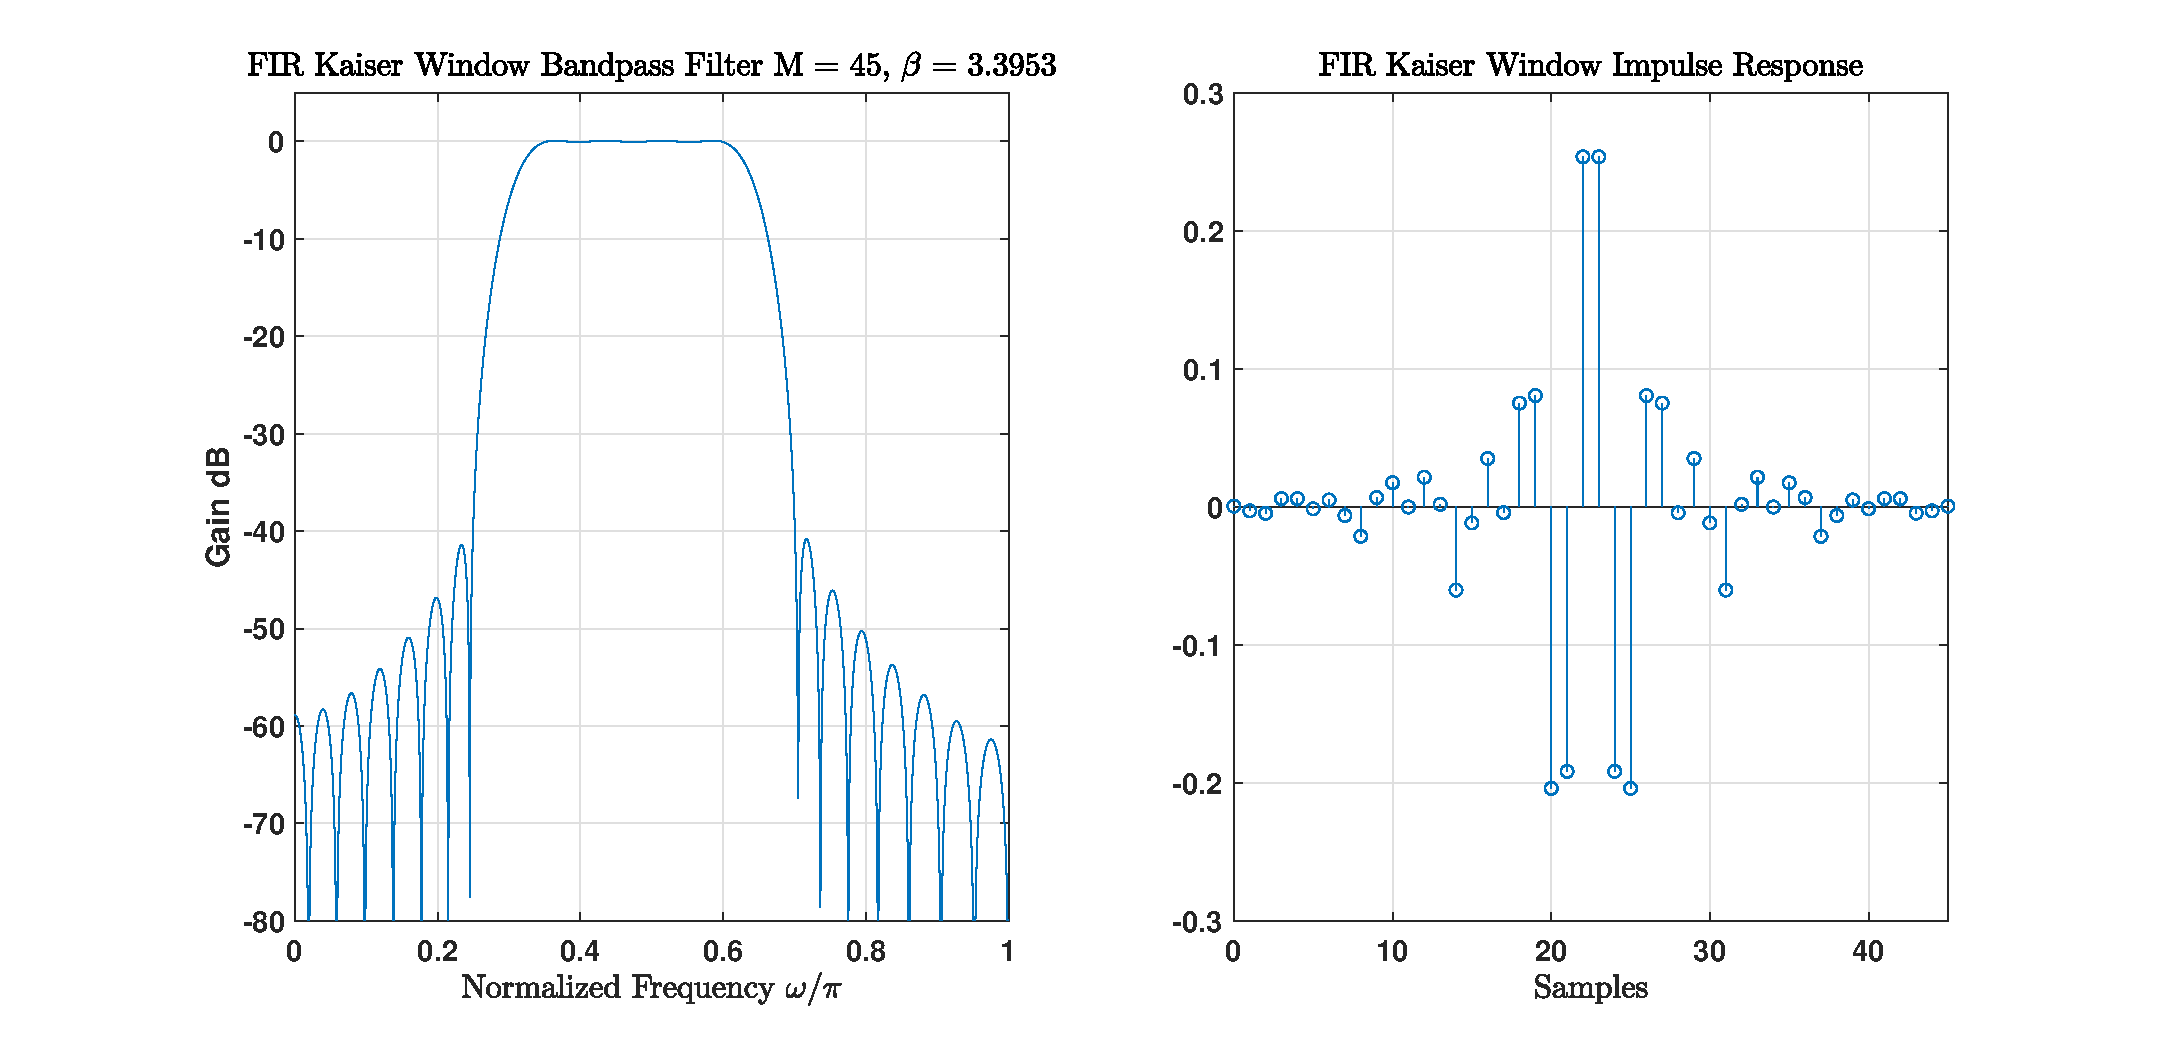
\includegraphics[scale = 0.5]{Figures/FIR_Sim/Bandpass_window_Kaiser.eps}
\caption{Bandpass Design Results for Kaiser Window}
\label{fig:FIR_Sim:bandpass_Kaiser_results}
\end{figure}

\begin{figure}[ht]
\centering
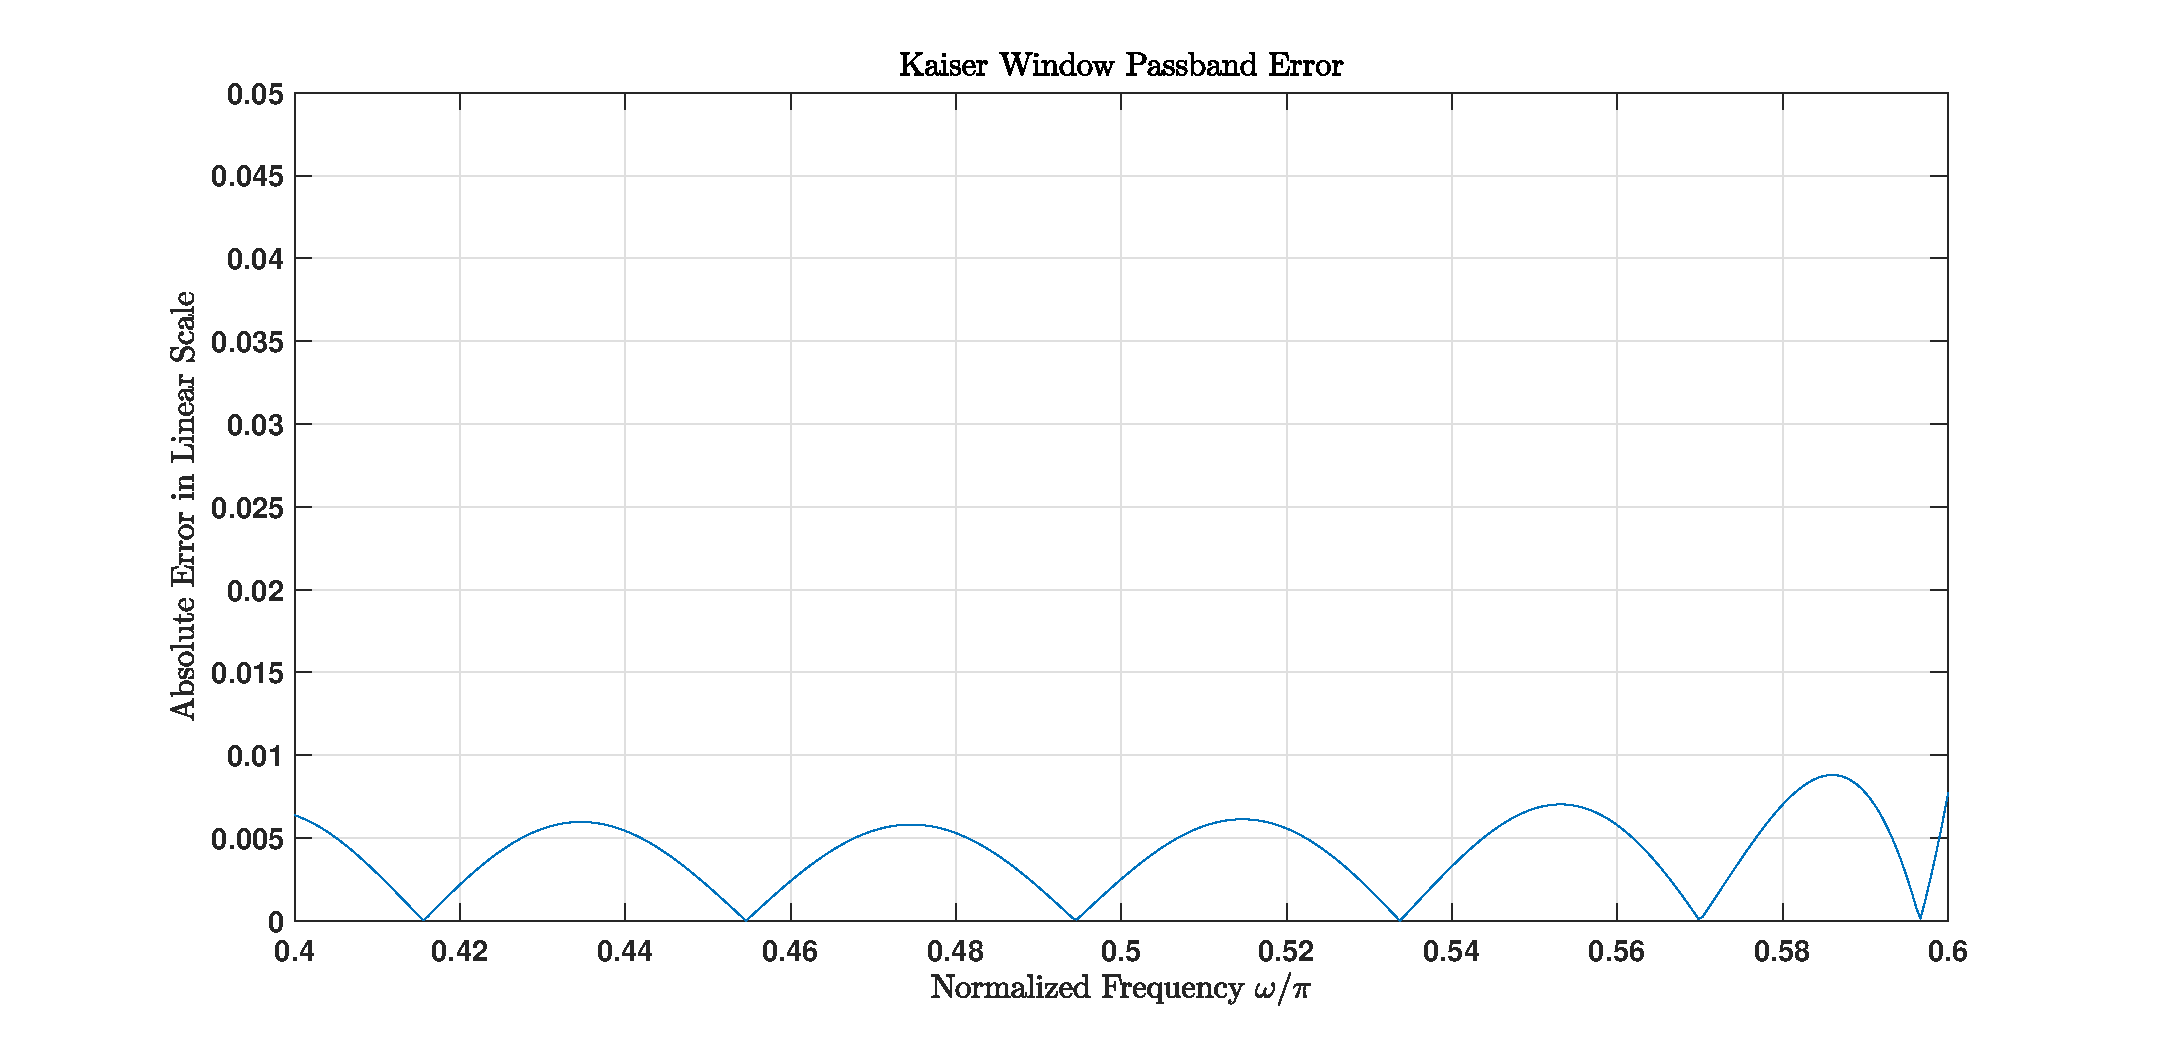
\includegraphics[scale = 0.3]{Figures/FIR_Sim/Bandpass_window_Kaiser_error_deviation.eps}
\caption{Bandpass Design Results for Kaiser Window: Error is less then 0.01}
\label{fig:FIR_Sim:bandpass_example_error_plot}
\end{figure}


\newpage
\section{Frequency Sampling Method}



\subsection{Low Pass Example}

The specifications are: 

\begin{itemize}

\item $\omega_{\text{pass}} \, = \, 0.25 \pi \, , \, \omega_{\text{stop}} \, = \, 0.35 \pi $

\item $  A_p \, = \, 0.1 \text{ dB} \, , \, A_s \, = \, 40 \text{ dB}$

\item By result the transition bandwidth is $\Delta \omega \, = \, \omega_{\text{pass}} \, - \, \omega_{\text{stop}} \, =  \, 0.35 \pi - \, 0.25 \pi  \, = \, 0.1 \pi$  


\end{itemize}


For a rectangular window as interpolating function, we have $\Delta \omega \, = \, \displaystyle\frac{4 \pi}{L} \rightarrow \, L \, = \, 40 \, = \, M \, + \, 1 $, so we need to begin with an \tbi{FIR of length at least 40} (order 39).\\



\begin{figure}[ht]
\centering
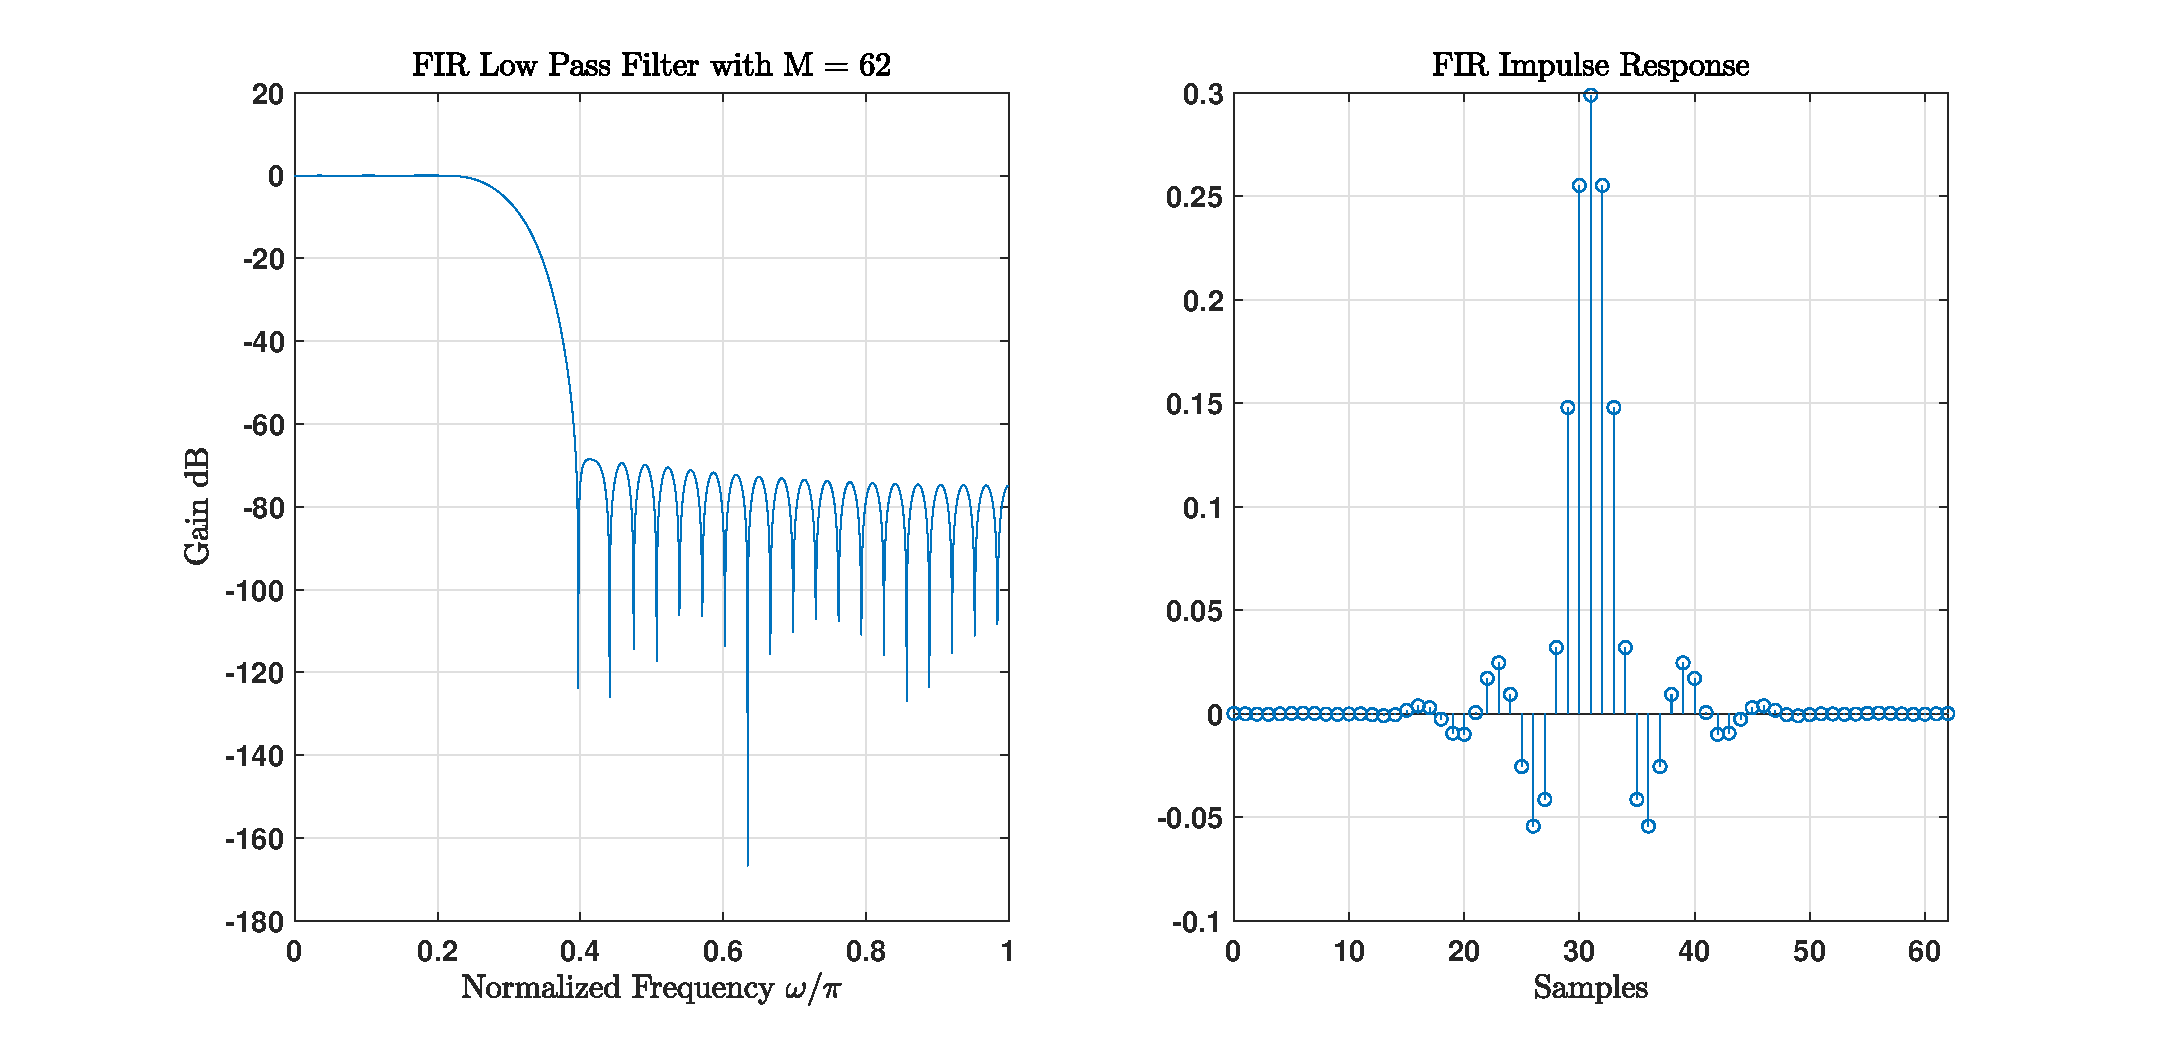
\includegraphics[scale = 0.4]{Figures/FIR_Sim/lowpass_freqsampling_method.eps}
\caption{FIR Low Pass with an order of $M\, = \, 62$}
\label{fig:FIR_Sim:lowpass_freqsampling_method}
\end{figure}



\todo{To do}:

\begin{itemize}

\item Write the formula and the design criteria

    \begin{itemize}
        \item Eq of FIR
        
        \item Steps of design in window method
        
        \item Concepts and techniques in designing
        
        \item Implementation using toolbox and from scratch
        
        \item Repeat the examples using toolbox and implementation using OOP style
        
        
    \end{itemize}

\end{itemize}